%========================================================================%
%               Copyright (C) 2016 All Rights Reserved.                  %
%             Author:BillHu<billhu@icloud.com>  Ver:<1.0>                %
%========================================================================%
%    The author grants permission, without fee and without a written     %
% license agreement, for use, reproduction, modification, and distribu-  %
% tion of this software and its documentation by educational, research,  %
% and non-profit entities for noncommercial purposes only.The above      %
% copyright notice and this paragraph MUST appear in all copies and      %
% modifications of the software and/or documentation.                    %
%========================================================================%
\documentclass{bjtu-bachelor-thesis}
%========================================================================%
% 自定义内容
%========================================================================%
\ctitle{基于\LaTeX 的毕设模板的设计与实现}
\etitle{The Design and Implementation of Thesis Template Based on \LaTeX}
\cauthor{张三}
\ctutor{刘四}
\cschool{软件学院}
\cmajor{软件工程}
\cid{18300704}

% 对应使用授权书下方的签名和日期,如果需要填写可改为
% \authorsign{张三}
% \tutorsign{刘四}
% \authorsigndate{2022年4月2日}
% \tutorsigndate{2022年4月2日}

\authorsign{\vspace{4ex}}
\tutorsign{\vspace{4ex}}
\authorsigndate{\hspace{2em}年\hspace{2em}月\hspace{2em}日}
\tutorsigndate{\hspace{2em}年\hspace{2em}月\hspace{2em}日}

%========================================================================%
% 自定义文字
%========================================================================%
\cthanks{放置在摘要页前,对象包括:1)国家科学基金,资助研究工作的奖学金基金,合同单位,资助或支持的企业、组织或个人。2)协助完成研究工作和提供便利条件的组织或个人。3)在研究工作中提出建议和提供帮助的人。4)给予转载和引用权的资料、图片、文献、研究思想和设想的所有者。5)其他应感谢的组织和个人。}
\cabstract{[鼠标左键单击选择该段落,输入替换之。内容为小四号宋体。] 中文摘要应将论文的内容要点简短明了地表达出来,约400字左右,字体为宋体小四号。内容应包括工作目的、研究方法、成果和结论。要突出本论文的创新点,语言力求精炼。为了便于文献检索,应在本页下方另起一行注明论文的关键词(3-5个),如有可能,尽量采用《汉语主题词表》等词表提供的规范词。图X幅,表X个,参考文献X篇。}
\eabstract{[鼠标左键单击选择该段落,输入替换之。内容为小四号Times New Roman。] 与中文摘要内容要相对应。``the'' quick brown fox jumps over the lazy dog}
\ckeywords{关键词1;关键词2;关键词3}
\ekeywords{KEYWORD1; KEYWORD2; KEYWORD3}
%========================================================================%
% 前置部分
%========================================================================%

\begin{document}
\pagenumbering{roman}
\cover % 封面
\ccopyright % 版权声明

\setcounter{page}{1}
\pagestyle{myfancy}

\cabspage % 中文摘要
\eabspage % 英文摘要

% 目录
\tableofcontents
\addcontentsline{toc}{part}{目\hspace{2em}录}%
\pagestyle{myfancy}
%========================================================================%
% 主体部份
%========================================================================%

\chapter{引言}
\pagestyle{myfancymain}
\setcounter{page}{1}
\pagenumbering{arabic}

[鼠标左键单击选择该段落,输入替换之。内容为小四号宋体。] 引言(或绪论)简要说明研究工作的目的、范围、相关领域的前人工作和知识空白、理论基础和分析、研究设想、研究方法和实验设计、预期结果和意义等。应言简意赅,不要与摘要雷同,不要成为摘要的注释。一般教科书中有的知识,在引言中不必赘述。
\chapter{【1级标题,三号黑体字】}
 [鼠标左键单击选择该段落,输入替换之。内容为小四号宋或楷体字。] 学位论文为了需要反映出作者确已掌握了坚实的基础理论和系统的专门知识,具有开阔的科学视野,对研究方案作了充分论证,因此,有关历史回顾和前人工作的综合评述,以及理论分析等,可以单独成章,用足够的文字叙述。正文是学位论文的核心部分,占主要篇幅,可以包括:调查对象、实验和观测方法、仪器设备、材料原料、实验和观测结果、计算方法和编程原理、数据资料、经过加工整理的图表、形成的论点和导出的结论等。\par
由于研究工作涉及的学科、选题、研究方法、工作进程、结果表达方式等有很大的差异,对正文内容不能作统一的规定。但是,必须实事求是,客观真切,准确完备,合乎逻辑,层次分明,简练可读。\par
\textcolor{red}{\textbf{图:}}\par
图包括曲线图、构造图、示意图、框图、流程图、记录图、地图、照片等。\par
图应具有“自明性”。\par
图应有编号。图的编号由“图”和从“1”开始的阿拉伯数字组成,图较多时,可分章编号。\par
图宜有图题,图题即图的名称,置于图的编号之后。图的编号和图题应置于图下方。\par
照片图要求主题和主要显示部分的轮廓鲜明,便于制版。如用放大缩小的复制品,必须清晰,反差适中。照片上应有表示目的物尺寸的标度。\par
图片示例1:
\begin{figure}[!htp]
    \centering
    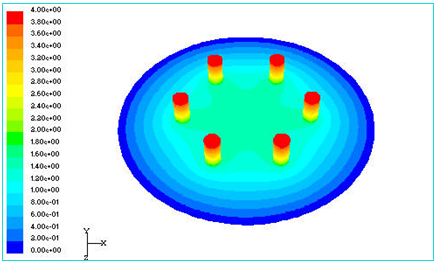
\includegraphics[width=0.5\textwidth]{pic/pic2-1.png}
    \caption{太合金多炭钢铁产品柱扭曲局部受力分析示意图\label{fig:2-1}}
\end{figure}

\textcolor{red}{\textbf{表:}}\par
表应具有“自明性”。\par
表应有编号。表的编号由“表”和从“1”开始的阿拉伯数字组成,表较多时,可分章编号。表较多时,可分章编号。表较多时,可分章编号。表较多时,可分章编号。\par
表宜有表题,表题即表的名称,置于表的编号之后。表的编号和表题应置于表上方。\par
表的编排,一般是内容和测试项目由左至右横读,数据依序竖读。\par
表的编排建议采用国际通行的三线表。\par
如某个表需要转页接排,在随后的各页上应重复表的编号。编号后跟表题(可省略)和“(续)”,置于表上方。\par
续表均应重复表头。\par
表格示例1:

\begin{table}[htbp]

    \centering
    \caption{国际单位制的基本单位}
    \label{tbl:2-1}
    \begin{tabularx}{0.8\textwidth}{*{3}{>{\centering\arraybackslash}X}}
        \toprule
        量的名称   & 单位名称     & 单位符号 \\ \midrule
        长度       & 米           & m        \\
        质量       & 千克(公斤)   & kg       \\
        时间       & 秒           & s        \\
        电流       & 安{[}培{]}   & A        \\
        热力学温度 & 开{[}尔文{]} & K        \\
        物质的量   & 摩{[}尔{]}   & mol      \\
        发光强度   & 坎{[}德拉{]} & cd       \\ \bottomrule
    \end{tabularx}
\end{table}

\textcolor{red}{\textbf{公式:}}\par
论文中的公式应另行起,并缩格书写,与周围文字留足够的空间区分开。\par
如有两个以上的公式,应用从“1”开始的阿拉伯数字进行编号,并将编号置于括号内。公式的编号右端对齐,公式与编号之间可用“…”连接。公式较多时,可分章编号。\par
公式示例1:
\begin{equation}
    \label{eqn:2}
    \phi=\frac{D_{p}^{2}}{150} \frac{\psi^{3}}{(1-\psi)^{2}}
\end{equation}
\begin{equation}
    \label{eqn:3}
    C_{2} =\frac{3.5}{D_{p}} \frac{(1-\psi)}{\psi^{3}}
\end{equation}

\noindent 式中  $\quad D_{p}$ —— 多孔质材料的平均粒子直径($m$);\par
$\psi$ —— 孔隙度(孔隙体积占总体积的百分比); \par
$\phi$ —— 特征渗透性或固有渗透性,与材料的结构性质有关($m^2$)。\par
较长的公式需要转行时,应尽可能在“=”处回行,或者在“+”、“-”“×”、“/”等记号处回行。\par
公式中分数线的横线,其长度应等于或略大于分子和分母中较长的一方。\par
如正文中书写分数,应尽量将其高度降低为一行。如将分数线书写为“/”,将根号改为负指数。\par
公式示例2:\par
\begin{spacing}{2}
    \begin{math}
        \zihao{5} \quad\text{将}\;\dfrac{1}{\sqrt{2}}\;\text{写成}\; 1/\sqrt{2} \;\text{或}\; 2^{-1/2}。
    \end{math}
\end{spacing}

\textcolor{red}{\textbf{引文标注}}\par
论文中引用的文献的标注方法遵照GB/T 7714-2005,可采用顺序编码制,也可采用著者-出版年制,但全文必须统一。\par
\textcolor{red}{\textbf{注释}}\par
当论文中的字、词或短语,需要进一步加以说明,而又没有具体的文献来源时,用注释。注释一般在社会科学中用得较多。\par
应控制论文中的注释数量,不宜过多。\par
由于论文篇幅较长,建议采用文中编号加“脚注”的方式。最好不用采用文中编号加“尾注”。\par

\section{【2级标题,小三号黑体字】 }
 [鼠标左键单击选择该段落,输入替换之。内容为小四号宋或楷体字。]
\subsection{【3级标题,四号黑体字】 }
[鼠标左键单击选择该段落,输入替换之。内容为小四号宋或楷体字。]

\chapter{【1级标题,三号黑体字】}
\section{【2级标题,小三号黑体字】 }
 [鼠标左键单击选择该段落,输入替换之。内容为小四号宋或楷体字。]
\subsection{【3级标题,四号黑体字】 }
[鼠标左键单击选择该段落,输入替换之。内容为小四号宋或楷体字。]

\chapter{【1级标题,三号黑体字】}
\section{【2级标题,小三号黑体字】 }
 [鼠标左键单击选择该段落,输入替换之。内容为小四号宋或楷体字。]
\subsection{【3级标题,四号黑体字】 }
[鼠标左键单击选择该段落,输入替换之。内容为小四号宋或楷体字。]

\chapter{结论【1级标题,三号黑体字】 }
 [鼠标左键单击选择该段落,输入替换之。内容为小四号宋或楷体字。] 论文的结论是最终的、总体的结论,不是正文中各段的小结的简单重复。结论应该准确、完整、明确、精练。如果不可能导出应有的结论,也可以没有结论而进行必要的讨论。可以在结论或讨论中提出建议、研究设想、仪器设备改进意见以及尚待解决的问题等。

\chapter{各种测试}
\section{图表测试}
\subsection{单张图片}
单张普通插图,及其引用,如图\ref{fig:G1}所示。

\begin{figure}[!htp]
    \centering
    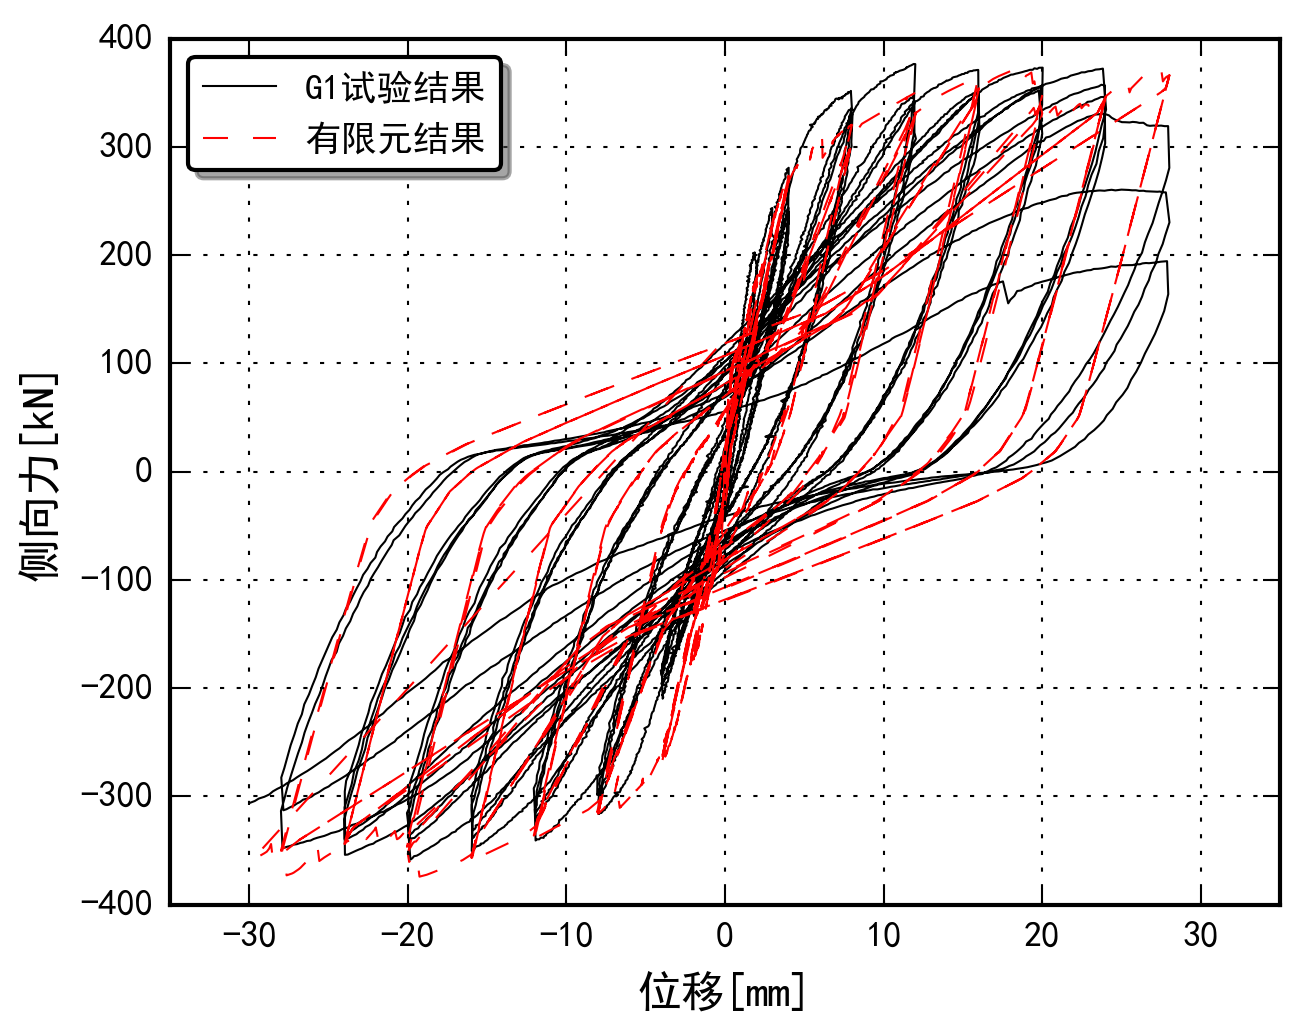
\includegraphics[width=0.8\textwidth]{pic/G1.png}
    \caption{G1数据对比\label{fig:G1}}
\end{figure}

\begin{figure}
    \centering
    \subcaptionbox{G1试件\label{fig:g1}}
    {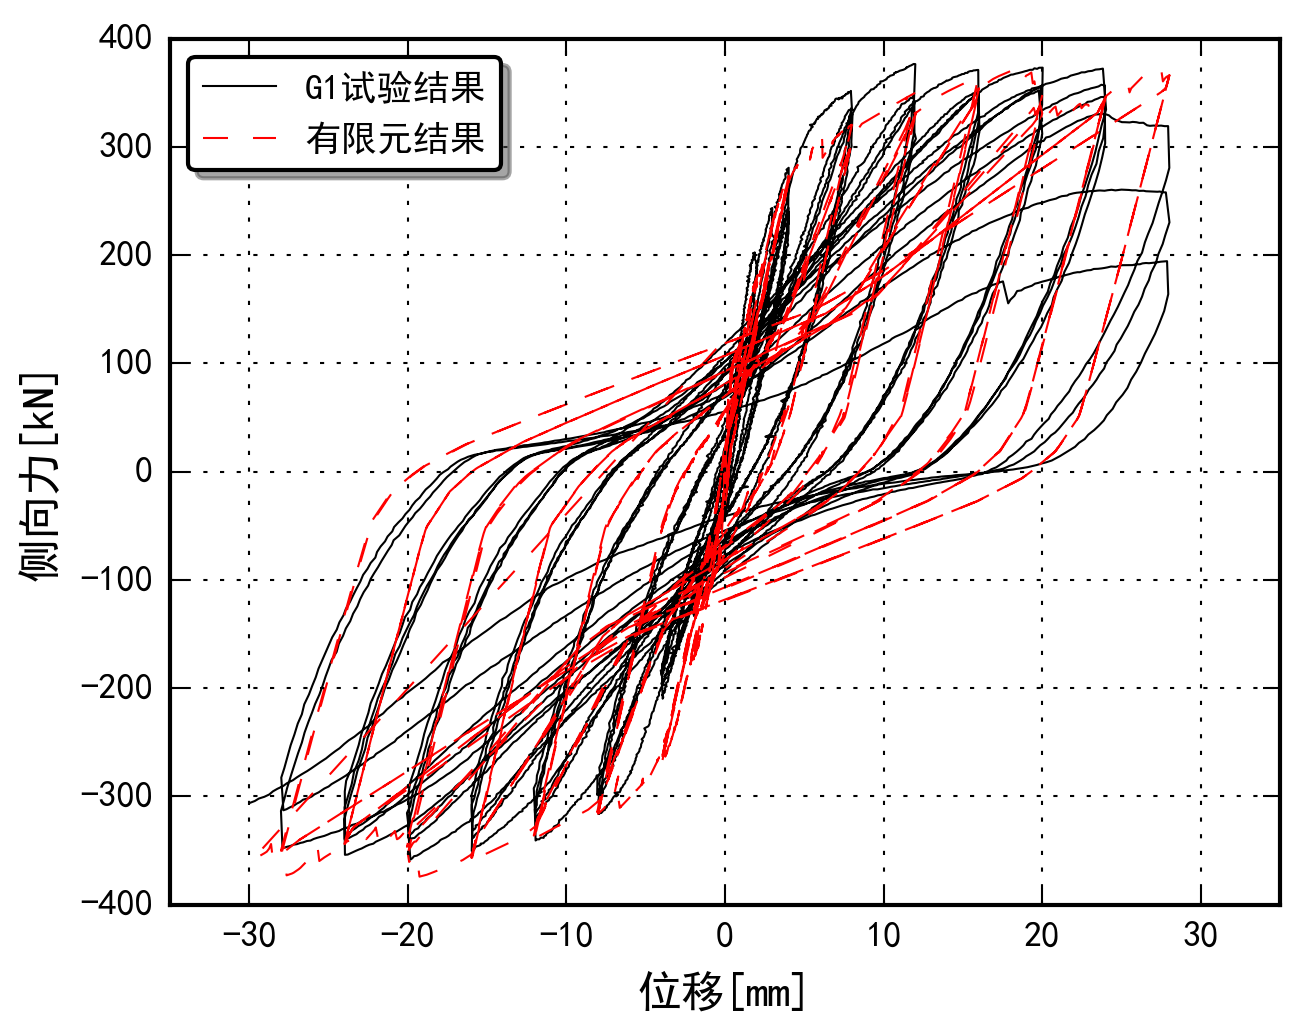
\includegraphics[width=0.4\textwidth]{pic/G1.png}}
    \subcaptionbox{G1试件\label{fig:g1-2}}
    {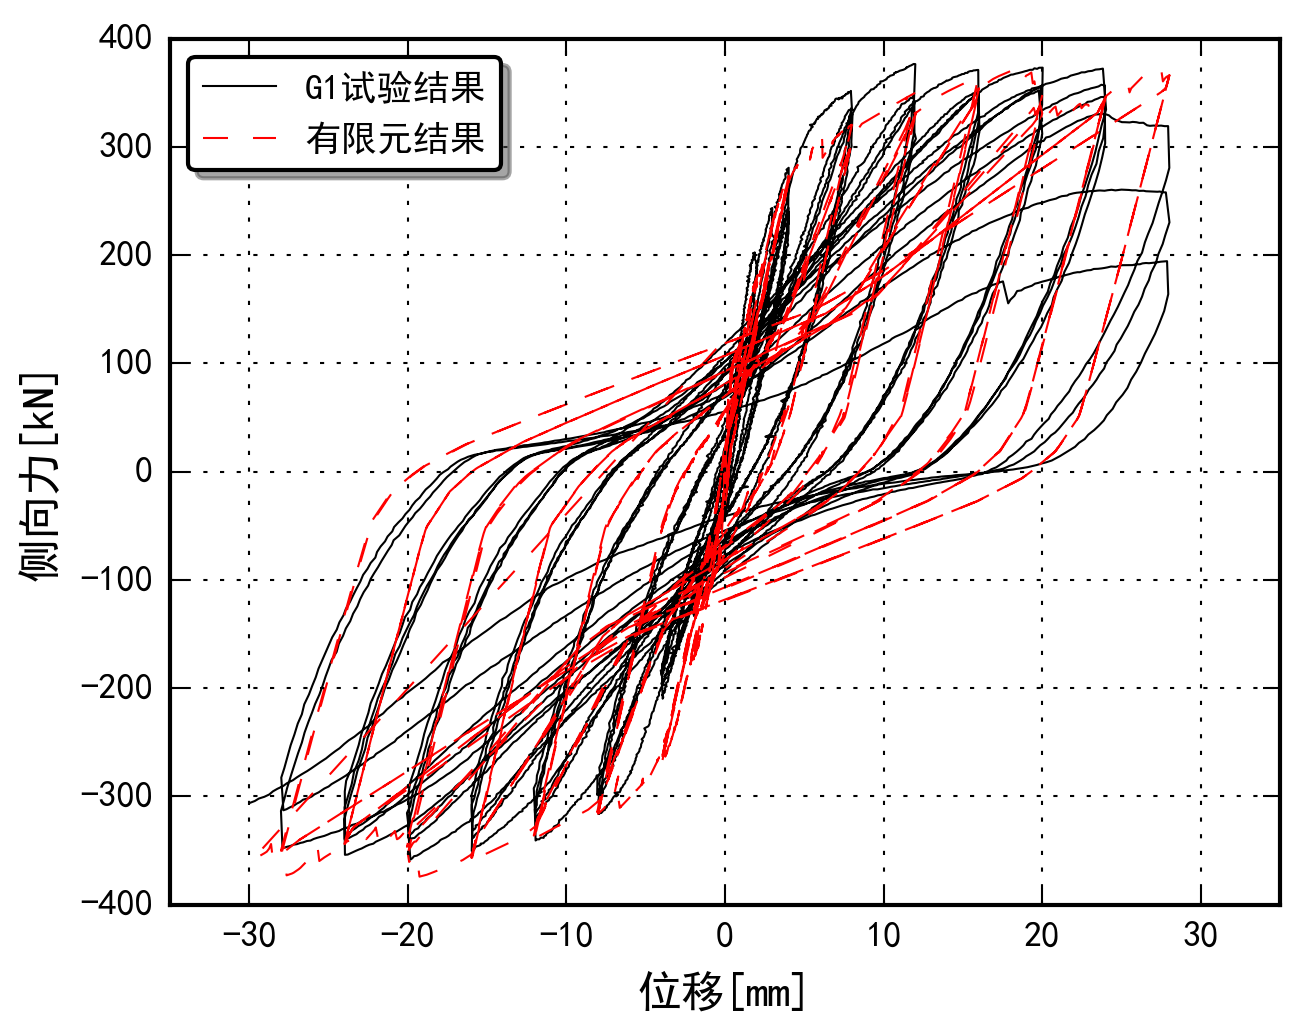
\includegraphics[width=0.4\textwidth]{pic/G1.png}}
    \caption{太合金多炭钢铁产品柱扭曲局部受力分析示意图}\label{fig:2}
\end{figure}

\section{公式测试}
公式的排版和引用与正常\LaTeX\ 公式格式一致。例如:

\begin{equation}
    \label{eqn:1}
    e^{i\pi}+1=0
\end{equation}

欧拉公式(式\ref{eqn:1}),它是数学里最令人着迷的一个公式,它将数学里最重要的几个数学联系到了一起——两个超数:自然对数的底$e$,圆周率$\pi$;两个单位:虚数单位$i$和自然数的单位$1$,以及数学里常见的$0$。数学家们评价它是“上帝创造的公式”,我们只能看它而不能理解它。

\section{参考文献测试}
我使用的参考文献是符合GB7714-2015规范的中文论文参考文献格式。该规范作为国家标准化管理委员会正式公布的标准,其权威性和通用性远远超过了其它格式规范,是国内最正式的参考文献格式规范,并且是大多数高校毕业论文和杂志的指定参考文献格式。

下面分类测试各种类型参考文献:

\begin{itemize}
    \item 中文规范\citep{C1}。
    \item 英文规范\citep{ACI318}
    \item 中文学位论文\citep{liguiqian}
    \item 英文学位论文\citep{bentz2000}
    \item 期刊\citep{FMK}
    \item 图书类\citep{B1}
    \item 其他\citep{R1}
    \item 多文献引用,压缩格式\citep{C1,ACI318,liguiqian,R1}
\end{itemize}

\begin{enumerate}
    \item one
    \item two
    \item ...
\end{enumerate}

\chapter{结论}
论文的结论是最终的、总体的结论,不是正文中各段的小结的简单重复。结论应该准确、完整、明确、精练。如果不可能导出应有的结论,也可以没有结论而进行必要的讨论。可以在结论或讨论中提出建议、研究设想、仪器设备改进意见以及尚待解决的问题等。
%========================================================================%
% 参考文献
%========================================================================%
\newpage
\pagestyle{myfancy}

% \nocite{*} % 显示.bib文件中的所有参考文献,无论正文是否引用

\printbibliography[heading=myheading]
\addcontentsline{toc}{part}{参考文献}
\cleardoublepage
%========================================================================%
% 致谢
%========================================================================%
\thankspage
%========================================================================%
% 附录
%========================================================================%
\markboth{附录}{}
% \let\cleardoublepage\relax
% \let\clearpage\relax
\addcontentsline{toc}{part}{附\hspace{2em}录}
\appendix

\chapter*{\makebox[\linewidth]{\zihao{-2}附\hspace{2em}录}}

\begin{appendices}
% \renewcommand{\thesubsection}{\Alph{subsection}}	
\section*{附录A\hspace{1em}外文文献原文}
\zihao{5}
\noindent MIPRO 2012, May 21-25,2012, Opatija, Croatia \par

\begin{center}
    A brief introduction to OpenCV\par
    Ivan Culjak, David Abram, Tomislav Pribanic, Hrvoje Dzapo, Mario Cifrek\par
    Faculty of electrical engineering and computing, University of Zagreb, Zagreb, Croatia\par
    ivan.culjak@fer.hr, david.abram@fer.hr, tomislav.pribanic@fer.hr,hrvoje.dzapo@fer.hr,mario.cifrek@fer.hr
\end{center}

\textbf{Abstract} - The purpose of this paper is to introduce and quickly make a reader familiar with OpenCV (Open Source Computer Vision) basics without having to go through the lengthy reference manuals and books. OpenCV is an open source library for image and video analysis, originally introduced more than decade ago by Intel. Since then, a number of programmers have contributed to the most recent library developments. The latest major change took place in 2009 (OpenCV 2) which includes main changes to the C++ interface. Nowadays the library has >2500 optimized algorithms. It is extensively used around the world, having >2.5M downloads and >40K people in the user group. Regardless of whether one is a novice C++ programmer or a professional software developer, unaware of OpenCV, the main library content should be interesting for the graduate students and researchers in image processing and computer vision areas. To master every library element it is necessary to consult many books available on the topic of OpenCV. However, reading such more comprehensive material should be easier after comprehending some basics about OpenCV from this paper. \par
\textbf{I. INTRODUCTION} \par
Computer Vision is the science of programming a computer to process and ultimately understand images and video, or simply saying making a computer see {[}1{]}. Solving even small parts of certain Computer Vision challenges, creates exciting new possibilities in technology, engineering and even entertainment. In order to advance vision research and disseminate vision knowledge, it is highly critical to have a library of programming functions with the optimized and portable code, and hopefully available for free. This was an original goal of Intel team back in 1999 when OpenCV (Open Source Computer Vision Library) was officially launched. Since then, a number of programmers have contributed to the most recent library developments. The latest major change took place in 2009 (OpenCV 2) which includes main changes to the C++ interface. The newest library release can be found on the OpenCV official website {[}2{]}. Nowadays the library has >2500 optimized algorithms. It is extensively used around the world, having >2.5M downloads and >40K people in the user group. OpenCV can be used in academic and commercial applications as well, under a BSD license {[}3{]}. To master every OpenCV library element it is necessary to consult many books available on the topic of OpenCV. Nevertheless, reading such more comprehensive material should be easier after comprehending a basic idea about OpenCV from this paper. In fact to make it even more convenient, the text presented here intentionally closely follows one of the most recent OpenCV sources {[}4{]}. \par
\textbf{II. BASIC LIBRARY STRUCTURE AND FEATURES} \par
OpenCV library (since version 2.2) is divided into several modules, where each module can be understood, in general, as being dedicated to one group of computer vision problems. All the classes and functions are defined within the name space cv. Therefore to access them we can either precede the main function definition by the declaration using namespace cv; or prefix OpenCV class and function names by namespace specification cv::. The main object is of class Mat. As implicated by the class name it is essentially a matrix holding pixel values of some image and, in addition, a number of attributes about an image. In the simplest case an image can be created as cv:: Mat image;, creating an image of size 0 by 0. Perhaps the most important member variable of image object is data where image.data member is actually a pointer to the allocated memory block that contains the image data (in this trivial case it would be image.data=0). Alternatively during a creation of Mat object we can explicitly specify an initial size and the type of each matrix element. This type specifies, for example, signed 1-byte pixel image values (CV\_8U), or three channels for a color image (CV\_8UC3), or even 32-bit/64bit floating point numbers (CV\_32F).\par
Once an object of class mat is defined, a nice feature about it (not present in the early versions of OpenCV) is that a memory allocation/deallocation takes place automatically. For instance, a memory automatically allocated during the image read out into some object, will be also automatically released once the corresponding object goes out of scope.\par
Another important thing is that Mat class implements the reference counting and shallow copy. Hence, when an image is assigned to another one, the image data itself is not copied and both images point to the same memory block (this also applies to images passed by/returned by value). However, since reference count is supported, a memory allocated for image (pixel) data itself will be released only when all of the references to the image are destructed.\par
In the versions prior to OpenCV 2, C like functions and structures were used (still can be though) and the main structure was IplImage. Although there is a convenient way to convert IplImage structure into cv::Mat object, it is highly recommended to avoid this deprecated data structure.\par

\section*{附录B\hspace{1em}外文文献翻译}

MIPRO 2012,2012年5月21日至25日,克罗地亚奥帕蒂亚
\begin{center}
    OpenCV简介\par
伊万·库尔贾克(Ivan Culjak),大卫·艾布拉姆(David Abram),托米斯拉夫·普里巴尼奇(Tomislav Pribanic),赫尔沃耶·德扎波(Hrvoje Dzapo),马里奥·奇夫雷克(Mario Cifrek)\par
克罗地亚·萨格勒布,萨格勒布大学·电气工程与计算学院\par
ivan.culjak@fer.hr,david.abram@fer.hr,tomislav.pribanic@fer.hr,rvoje.dzapo@fer.hr,mario.cifrek@fer.hr\par
\end{center}

\textbf{摘要}——本文的目的是介绍并使读者快速熟悉OpenCV(开源计算机视觉库)的基础知识,而无需翻阅冗长的用户手册和书籍。OpenCV是一个开源的、用于图像和视频分析的库,最初由英特尔在十几年前提出。从那以后,大量程序员对最新的这版库做出了贡献。最新的重大变化发生在2009年(OpenCV 2版本),这一版本包含了对C ++接口的主要修改。如今这个库有超过2500个优化算法。它被广泛用于全球各地,下载量超过250万,用户组超过4万人。对于研究图像处理和计算机视觉领域的研究生和研究人员而言,不管是C ++的新手程序员还是专业软件开发人员,很少不知道OpenCV,这个领域的主要的库内容。要想掌握每一个库元素,有必要查阅许多OpenCV领域的书籍。但是,理解本文中有关OpenCV的一些基础知识后,再去读更全面的材料应该会更容易。\par
\textbf{一、简介} \par
计算机视觉是一门编写计算机程序来处理并最终理解图像和视频,或者简单说来,让计算机可以“看到”的科学。哪怕解决计算机视觉的很小一部分挑战,就可以在技术,工程学甚至娱乐领域创造令人兴奋的新机遇。为了推进视觉研究并传播视觉知识,建立一个优化的、可移植的,而且最好是可以免费使用的程序函数的代码库是非常必要的。时间倒流回1999年,OpenCV(开源计算机视觉库)正式发布的时候,这就是英特尔团队最初的目标。从那时起,许多程序员为最新一版的库的开发做出了贡献。最新的重大变化发生在2009年(OpenCV 2)发布的时候,它包含了对C++接口的主要更改。最新的库的发行版可以在OpenCV的官方网站上找到。如今,该库有2500多个优化算法。它在世界范围内被广泛使用,下载量超过250万,用户数量超过4万。OpenCV可用于学术领域,也可以在BSD许可下用于商业领域。要想掌握每一个库元素,有必要查阅许多OpenCV领域的书籍。但是,理解本文中有关OpenCV的一些基础知识后,再去读更全面的材料应该会更容易。实际上,为了使它更加易读,这里的用语和措辞遵循最新的OpenCV源码版本之一。\par
\textbf{二、库的基本结构和特性} \par
OpenCV库(自版本2.2起)分为几个模块,通常情况下,每个模块都可以理解为专用于解决一组计算机视觉的问题。所有的类和函数都已定义在命名空间cv中。因此,为了访问它们,我们可以在主函数定义之前加上using namespace cv;或在OpenCV类和函数名称前加前缀,通过命名空间cv ::声明。主要的对象是Mat类。就像类名所提示的那样,它本质上是一个矩阵,用于存放一些图像的像素值,此外,还有一些图像的基本属性。在最简单的情况下,可以将图像创建为cv :: Mat image;,这就创建了一个大小为0 x 0的图像。image对象最重要的成员变量是data, image.data成员实际上是指向分配的包含图像数据的内存块的指针(在这种简单的情况将是image.data= 0)。另外,在创建Mat对象的过程中,我们可以显式指定每个矩阵元素的初始大小和类型。例如可以指定,带符号的1字节像素图像值(CV\_8U),或彩色图像的三个通道(CV\_8UC3),甚至32位/ 64位浮点数(CV\_32F)。
定义了mat类的对象后,它的一个很好的特性是(在早期版本的OpenCV中不存在)是自动进行内存分配/释放。例如,在图像读取期间内存自动分配到某个对象中,同时,一旦对应对象超出生命周期,也会自动释放。\par
另一个重要的事情是Mat类实现了参考计数和浅表复制。因此,当图像内容被分配给另一个图像,图像数据本身并未复制,两个图像都指向相同的内存块(这也适用于传递/返回的图像值)。但是,由于支持引用计数,因此分配给图像(像素)数据本身的内存仅当所有对图像的引用均被销毁时才释放。
在OpenCV 2之前的版本中,类似C的函数和结构被使用(虽然仍然可以),主要结构是IplImage。虽然有一个将IplImage结构转换为cv :: Mat对象的便捷方法,但是强烈建议避免使用不推荐的数据结构。\par
\end{appendices}

\end{document}
